% !TeX root = ../tesis.tex


\chapter{Ajuste con el modelo de Lorentz}

\label{section:apendix1}

En la sección \ref{section:optical_properties} se obtuvo una expresión analítica de la parte imaginaria de la función dieléctrica de los eritrocitos y el plasma a través de un ajuste con el modelo de Lorentz. En esta sección se mostrarán los valores empleados para los ajustes con el modelo de Lorentz así como las gráficas de los ajustes obtenidos.
\vspace{-0.5cm}
\begin{itemize}
	\item Concentración 15.3 g/dL
	\begin{table}[h!]
		\centering
		\setlength{\tabcolsep}{12pt} 

		\begin{tabular}{ccccc}
			\hline
			% Encabezado con color personalizado
		$i$ & $A_i\, [\text{eV}]^2$  & $\hbar\omega_i$ [eV] & $\hbar\gamma_i$ [eV] \\
			\hline
			1 & $4.13 \times 10^{-4}$ & 2.16 & $5.61 \times 10^{-2}$ \\
			2 & $6.64 \times 10^{-4}$ & $2.29$ & $9.01 \times 10^{-2}$ \\
			3 & $1.39 \times 10^{-2}$ & $3$ & $1.86 \times 10^{-2}$ \\
			4 & $6.55 \times 10^{-3}$ & $3.59$ & $5.14 \times 10^{-1}$\\
			5 & $1.76 \times 10^{-2}$ & $4.6$ & $8.32 \times 10^{-1}$ \\
			6 & $1.15 \times 10^{-5}$ & $2.72$ & $7.83 \times 10^{-3}$ \\ \hline
		\end{tabular}
		\caption{Parámetros del modelo de Lorentz empleados para una CHCM de 15.3 g/dL.}
		
	\end{table}
	%
	\begin{figure}[h!]
		\centering
		\includegraphics[width=0.7\textwidth]{../../Figuras/ajusteLorentz15.pdf}
		\caption{Parte imaginaria de la función dieléctrica de eritrocitos con una CHCM de 15.3 g/dL. Los datos experimentales se obtuvieron de \cite{friebelDeterminationComplexRefractive2005a} y están indicados mediante puntos rojos. La línea azul continua representa el ajuste con lorentzianas obtenido. Las líneas grises verticales indican las frecuencias de resonancia asociadas a los osciladores de Lorentz empleados en el ajuste.}
		\label{fig:lorentz15}
	\end{figure}
	%
	
	\item Concentración 28.7 g/dL
	\begin{table}[h!]
		\centering
		\setlength{\tabcolsep}{12pt} 
		% Alterna blanco y un azul muy clarito para que los datos sean legibles
		
		
			\begin{tabular}{ccccc}
			\hline
			% Encabezado con color personalizado
			$i$ & $A_i\, [\text{eV}]^2$  & $\hbar\omega_i$ [eV] & $\hbar\gamma_i$ [eV] \\
			\hline
			1 & $4.87 \times 10^{-4}$ & 2.14 & $5.23 \times 10^{-2}$ \\
			2 & $8.28 \times 10^{-4}$ & $2.27$ & $9.33 \times 10^{-2}$ \\
			3 & $1.8 \times 10^{-2}$ & $3.01$ & $1.87 \times 10^{-1}$ \\
			4 & $8.47 \times 10^{-3}$ & $3.61$ & $5.23 \times 10^{-1}$\\
			5 & $1.84 \times 10^{-2}$ & $4.58$ & $7.37 \times 10^{-1}$ \\
			6 & $2.66 \times 10^{-5}$ & $2.72$ & $1.44 \times 10^{-2\underline{}}$ \\ \hline
		\end{tabular}
		\caption{Parámetros del modelo de Lorentz empleados para una CHCM de 28.7 g/dL.}
	\end{table}
	%
	\begin{figure}[h]
		\centering
		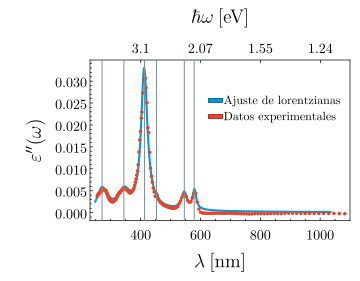
\includegraphics[width=0.47\textwidth]{../../Figuras/ajusteLorentz28.pdf}
		\caption{Parte imaginaria de la función dieléctrica de eritrocitos con una CHCM de 28.7 g/dL. Los datos experimentales se obtuvieron de \cite{friebelModelFunctionCalculate2006} y están indicados mediante puntos rojos. La línea azul continua representa el ajuste con lorentzianas obtenido. Las líneas grises verticales indican las frecuencias de resonancia asociadas a los osciladores de Lorentz empleados en el ajuste.}
		\label{fig:lorentz28}
	\end{figure}
	%
	
	
	\item Concentración 30.6 g/dL
	\begin{table}[h!]
		\centering
		\setlength{\tabcolsep}{12pt} 
		% Alterna blanco y un azul muy clarito para que los datos sean legibles
		
		
		\begin{tabular}{ccccc}
		\hline
		% Encabezado con color personalizado
		$i$ & $A_i\, [\text{eV}]^2$  & $\hbar\omega_i$ [eV] & $\hbar\gamma_i$ [eV] \\
		\hline
		1 & $3.86 \times 10^{-4}$ & 2.16 & $5.41 \times 10^{-2}$ \\
		2 & $6.96 \times 10^{-4}$ & $2.29$ & $9.99 \times 10^{-2}$ \\
		3 & $1.51 \times 10^{-2}$ & $3$ & $9.99 \times 10^{-2}$ \\
		4 & $1.51 \times 10^{-2}$ & $3$ & $2.08 \times 10^{-1}$\\
		5 & $6.08 \times 10^{-3}$ & $3.6$ & $5.1 \times 10^{-1}$ \\
		6 & $1.82 \times 10^{-2}$ & $4.61$ & $8.75 \times 10^{-1}$ \\ \hline
	\end{tabular}
		\caption{Parámetros del modelo de Lorentz empleados para una CHCM de 30.6 g/dL.}
		
	\end{table}
	
	%
	\begin{figure}[h]
		\centering
		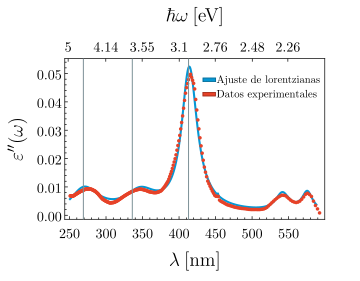
\includegraphics[width=0.7\textwidth]{../../Figuras/ajusteLorentz30.pdf}
		\caption{Parte imaginaria de la función dieléctrica de eritrocitos con una CHCM de 15.3 g/dL. Los datos experimentales se obtuvieron de \cite{friebelDeterminationComplexRefractive2005a} y están indicados mediante puntos rojos. La línea azul continua representa el ajuste con lorentzianas obtenido. Las líneas grises verticales indican las frecuencias de resonancia asociadas a los osciladores de Lorentz empleados en el ajuste.}
		\label{fig:lorentz30}
	\end{figure}
	%
	
	
	
\end{itemize}